\subsection{MVC}
Since the 1970s the Model View Controller ( MVC ) pattern is the standard architectural design pattern for applications that present the user with a graphical user interface. It was developed out of a need for modularity, to encapsulate responsibility of specific concepts to separate program modules, or Separation of Concerns. MVC identifies three main components that program code should be grouped into, namely\cite{walther_2016}:

\begin{itemize}[label={}]

\item \textbf{Model}: The representation of some object of knowledge, encapsulates code managing the associated data and behaviour ( business-logic ).
\item \textbf{View}: The visual representation of the model. The view can feature or hide aspects of the model and thus act as a presentation filter. The view observe the model for changes and update the presentation accordingly.
\item \textbf{Controller}: The controller allows the user to interact with the model. It allows the user to trigger behaviours implemented in the Model.

\end{itemize}

In the classic MVC pattern the model does not "know" about the view or the controller. And the controller does not effect the view. Instead, both the view and controller monitor the model using an observer mechanism and synchronise themselves when updates to the model occur.

\begin{figure}[H]
    \centering
    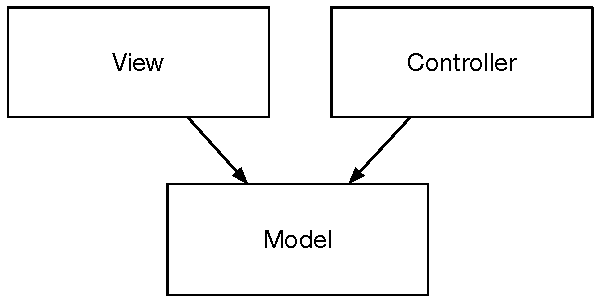
\includegraphics[height=4cm,keepaspectratio]{assets/concept/mvc_1.pdf}
    \caption{Classic MVC}
    \label{fig:mvc_1}
\end{figure}

\subsection{Modern MVC}

Modern MVC has evolved from being a software design pattern which handles components of an application to an architectural design pattern that defines the structure of an application itself. It has many similarities to the Layer Architecture. The responsibilities of each layer are slightly different to the typical presentation, business, and persistence layer definitions.

Most modern web frameworks such as Ruby on Rails, Symfony or the IOS environment refer to themselves as MVC based frameworks. The modern MVC concept has changed slightly. The component definitions are the same, but some responsibilities have shifted. Modern MVC strictly separates the model from the view. All modern frameworks state that the view should have as little logic as possible. Any logic implemented in the view should only be relevant to presentation. The view components should not directly reference the model components\cite{apple_MVC}\cite{symfony_MVC}.

\begin{figure}[H]
    \centering
    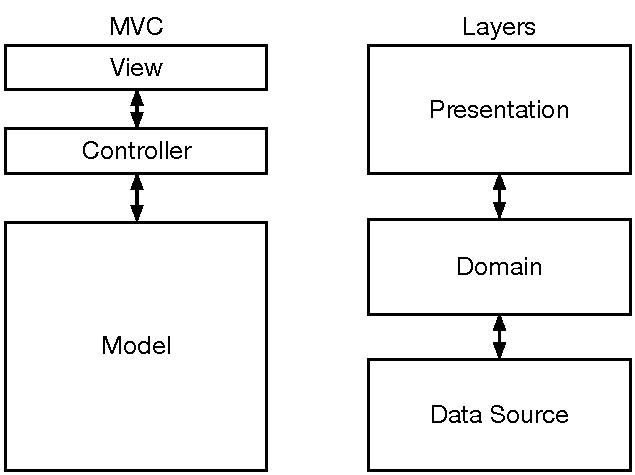
\includegraphics[height=4cm,keepaspectratio]{assets/concept/mvc_2.pdf}
    \caption{Modern MVC vs 3-Tier Layered Architecture}
    \label{fig:mvc_2}
\end{figure}

This division of responsibility has the added benefit of increased testability. GUIs are difficult to test, by removing as much logic as possible from the user interface there is less necessity to test it. The controller and model components can more easily be tested independently of one another using normal unit tests\cite{mvp_testing}.

\subsection{MVC Derivatives}

Many MVC derivatives exist. The main differences are where the division of responsibility is made and how it is labeled. MVVM defines a view model instead of a controller. The view model acts as a facade around the model and introduces a data binder element that is responsible for keeping the view and view model synchronised. The MVT, calls the view a template and the controller a view. The slight difference is that the template is basically a static file, with no logic, and placeholders for the data. The Django web framework uses this model, but there is little difference to the other MVC derivatives such as MVP ( model view presenter ). The AngularJS web framework takes ends the discussion of which design to follow by labelling itself a MVW ( model view whatever ) framework\cite{mvw}.


\begin{figure}[H]
    \centering
    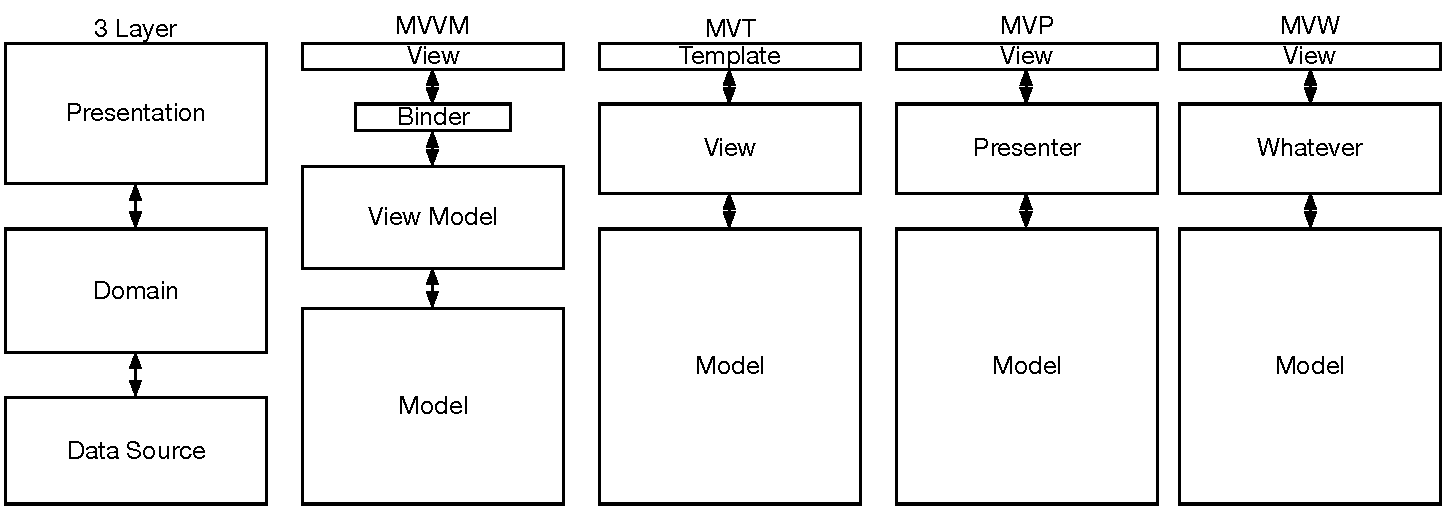
\includegraphics[height=4cm,keepaspectratio]{assets/concept/mvc_3.pdf}
    \caption{MVC Derivatives Overview}
    \label{fig:mvc_alt}
\end{figure}

\subsection{MVC and Smart Phone Applications}

Although most frameworks and environments targeted toward mobile application development use concepts from MVC, it can be difficult to define strict devision of responsibility, especially in conjunction with services provided from an online server. Often the responsibilities of the controller are reimplemented server side, some model management might occur in the app. Server and application code are developed using different languages and often most likely different developers. One solution is is to develop the app as a thin client, where it basically becomes the view component of MVC and the controllers and model are implemented on the server. Taken to the extreme, the app runs in a standard web browser and server provides the view components that emulate a native mobile user interface. This is referred to as a web app. Any logic in the view is implemented using javascript. Hardware support is limited to what the mobile browser provides access to. In order to extend hardware support a hybrid approach can be used in which the app implements a custom browser view which is extended with native capabilities. Here is division or responsibilities as defined by MVC become fuzzy. A fully native app working in conjunction with a web server will not conform well to the definitions of MVC.

\subsection{VIPER}

VIPER is a new software architecture pattern which extends MVC with some addition concepts that make it more adaptable to mobile applications, especially when they are extended with online server based services. The classic controller is split into a presenter and a controller, the model component is split into a central data manager communicating with many services and entities\cite{viper}.

\begin{figure}[H]
    \centering
    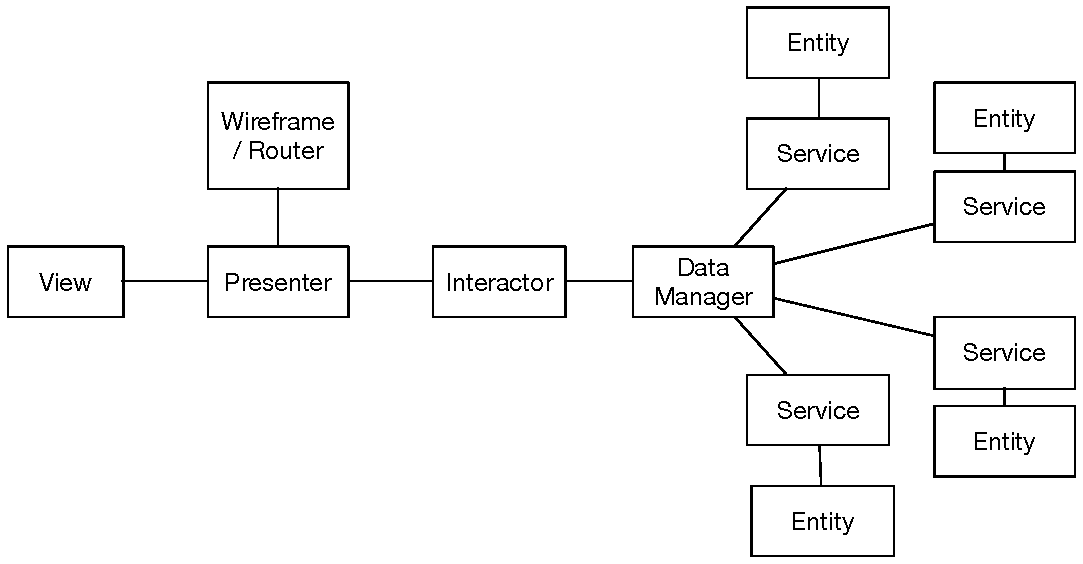
\includegraphics[height=6cm,keepaspectratio]{assets/concept/viper.pdf}
    \caption{VIPER Overview}
    \label{fig:viper}
\end{figure}

\begin{itemize}[label={}]

\item \textbf{View}: The view corresponds to the view as defined in modern MVC definitions, it is a slim component with as little logic as possible. It presents the current state of the models and provides “widgets” with which the user can interact.
\item \textbf{Presenter}: The presenter passes data to the view and handles events from the view. The presenter might perform some basic validation, in the case of a user sign-up scenario, for example, the presenter might validate that a user’s email is indeed formatted as a correct email, it will not validate if the email has already been used by someone else.

\item \textbf{Interactor}: Business logic is handled by the interactor. Most a what the model component in MVC was responsible for is handled here. The interactor however does not know anything about data storage, databases, or persistence. It does not know if data is local or accessible via a network.

\item \textbf{Data Manager}:
\item \textbf{Service}:
\item \textbf{Entity}:
\item \textbf{Wireframe / Router}:

\end{itemize}